%!TEX root = ../../../report.tex
\section{Project management} % (fold)
\label{sec:project_management}
The methodology used for this project is Agile.
Agile approaches help teams respond to unpredictability through incremental, iterative work cadences, known as sprints.
It has been implemented as SCRUM \cite{singh2008u} by considering both supervisors as the product managers and having a self managed team striving to build properly tested product increments within short iterations.
By having weekly meetings, empirical feedback has been received closing the iteration circle faster and more concisely.

The tool Trello \cite{trello} has been used in order to keep track of the tasks in the backlog.
Trello is an online project management application and it was used since its design made it similar to post-it notes for management.
It also has the advantage of being online and therefore accessible from both home and workplace through smart phones or computers.
Figure \ref{fig:trello} shows a screen capture of Trello board for a sprint log.

\begin{figure}[ht]
  \centering
  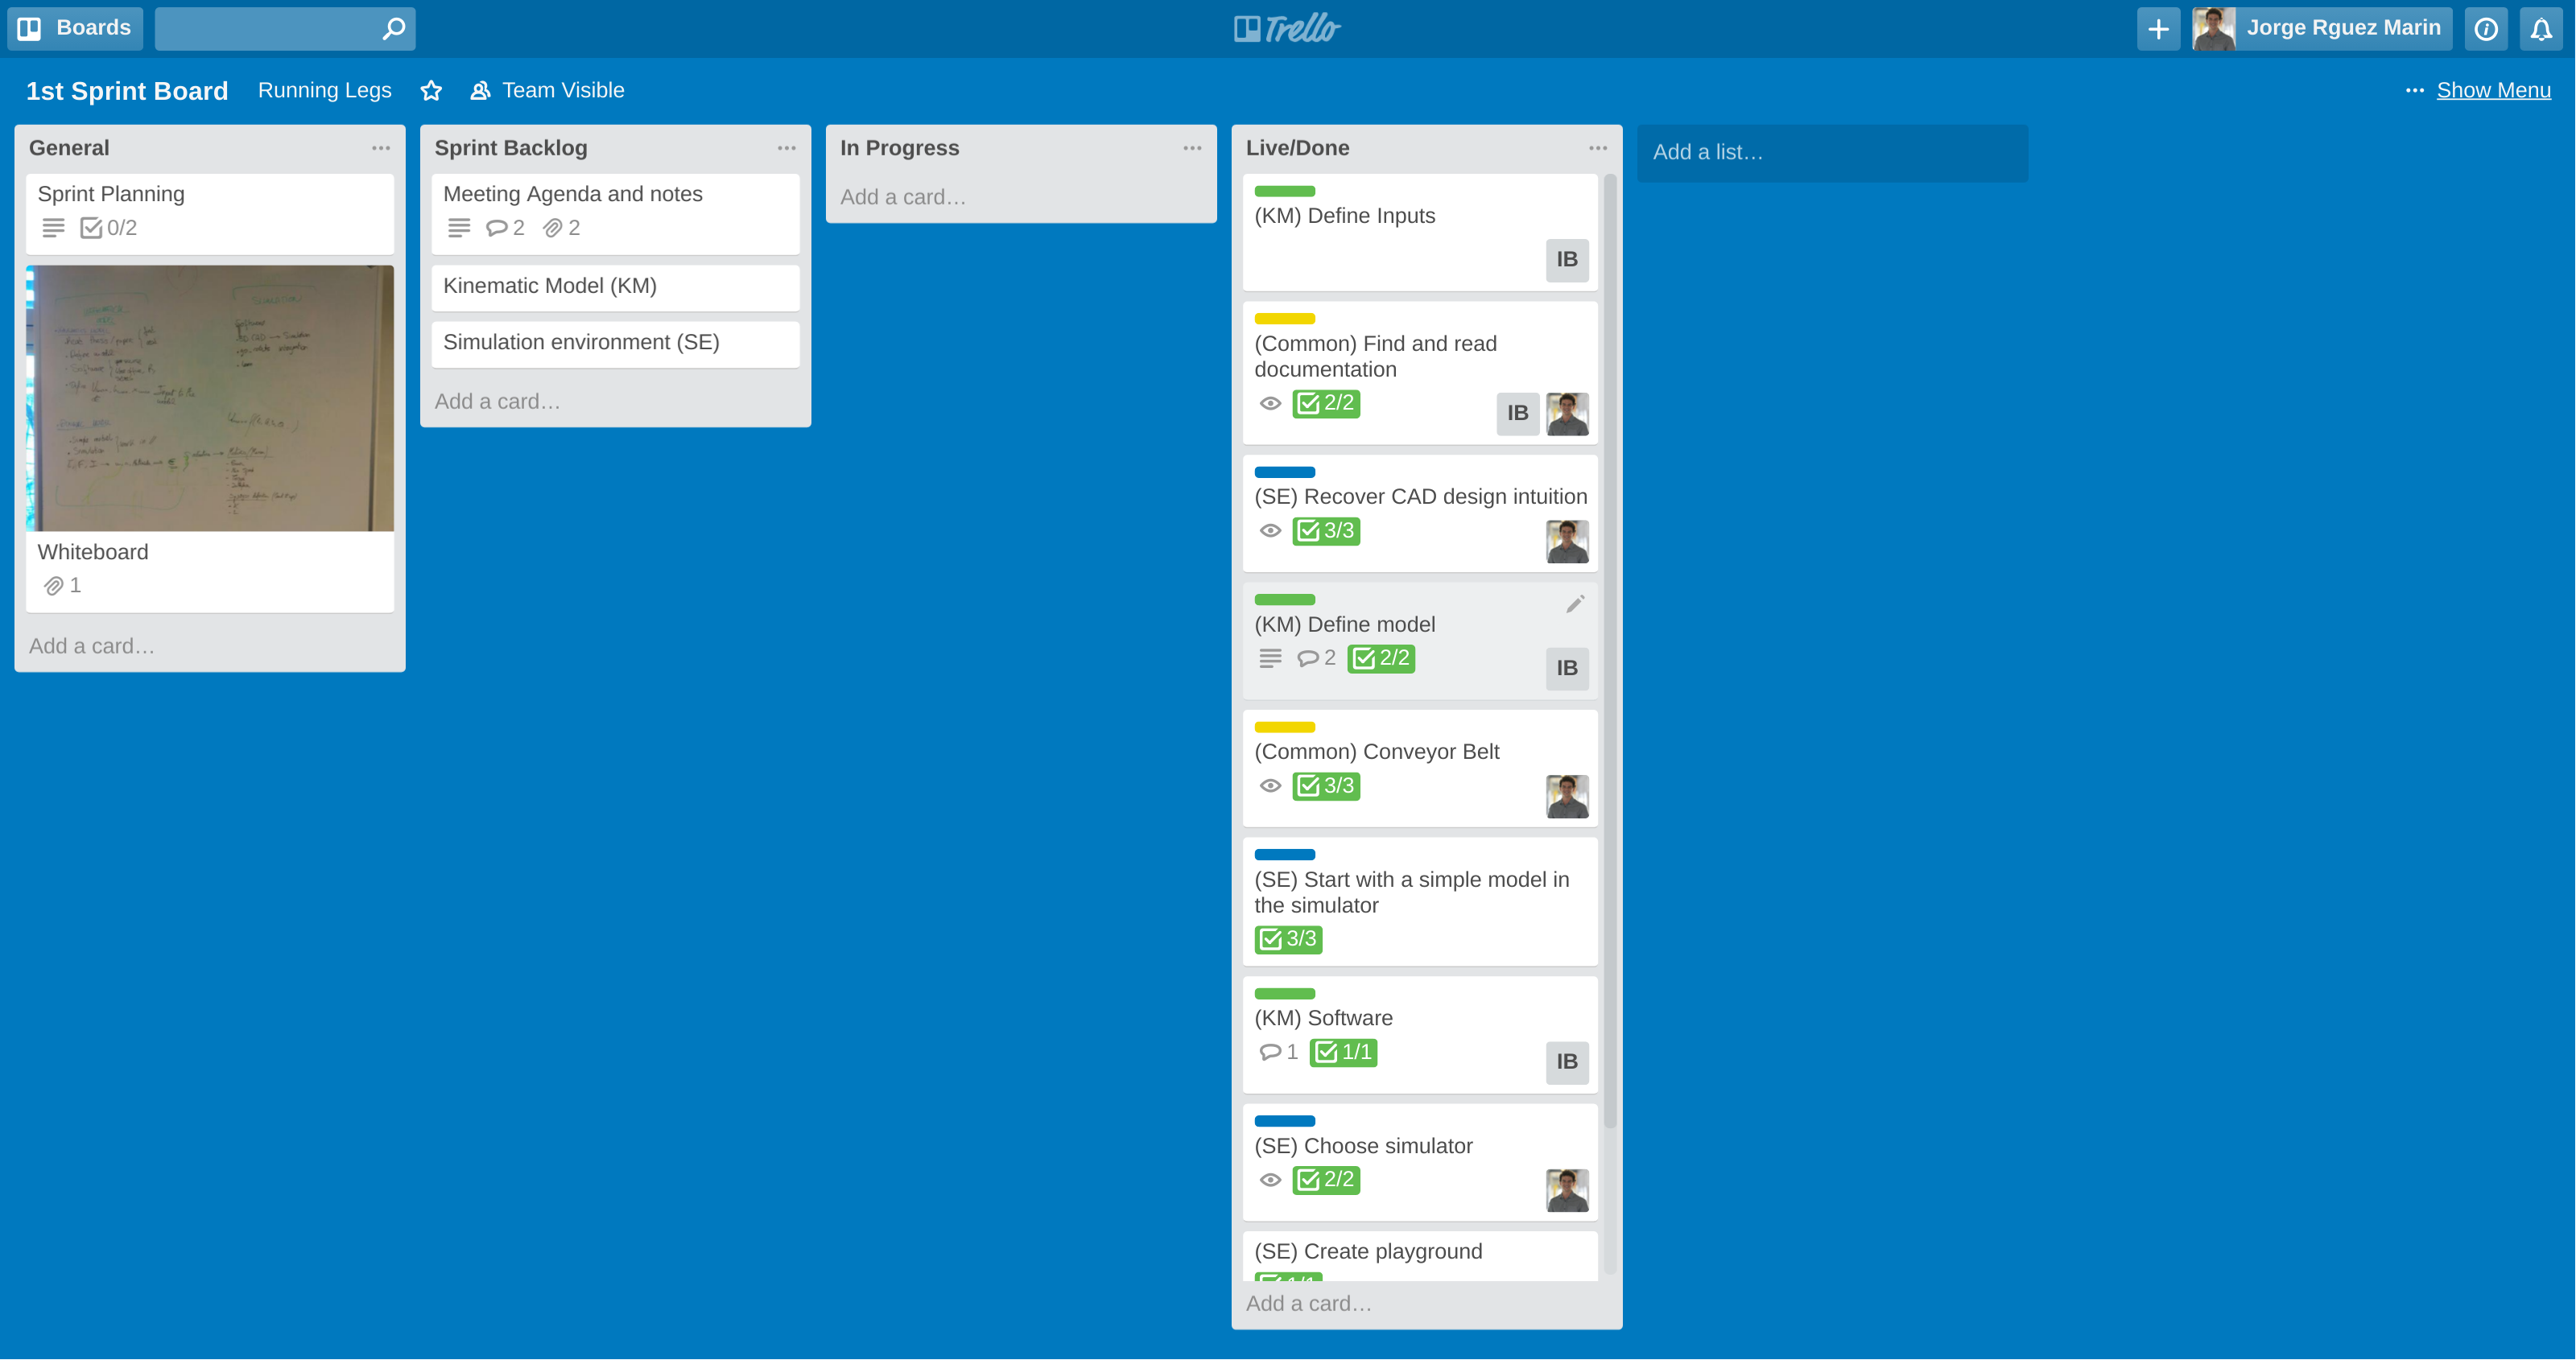
\includegraphics[width=\textwidth]{figures/trello.png}
  \caption{Screen capture of Trello showing the 1st sprint board. The three
rightmost lists are used to keep track of tasks and their state.}
  \label{fig:trello}
\end{figure}

Besides, the project has been organized in four sprints with big tasks that then are broken down into smaller jobs. The sprints are:
\begin{enumerate}
  \item \textbf{Sprint 1}
    \begin{itemize}
      \item \textbf{Goal}: Analyze robot possibilities, define the kinematic model, become familiar with the simulation environment and get ready ROS Control and software.
      \item \textbf{Duration}: 21st of January to 28th of February
      \item \textbf{Description}: An analysis of the structural possibilities of the robots is done. This is then used to start the mathematical model, which is subdivided in the kinematic and the dynamic model so the first one can be started. In parallel, all the software environment is created: from ROS control to the Gazebo structures. This will help with future extensions and will facilitate its integration for new features like the real CAD model of the robot.
    \end{itemize}
    \item \textbf{Sprint 2}
    \begin{itemize}
      \item \textbf{Goal}: Define the dynamic model, integrate Go Robots in the software structures and prepare simple simulation for testing and create example controllers.
      \item \textbf{Duration}: 3rd of March to 1st of April
      \item \textbf{Description}: The kinematic model is finished and the dynamic starts. From the software point of view, a basic simulation model is created and controlled with ROS Control. The example controllers, based on tools from Go Robots, are created and tested.
    \end{itemize}
  \item \textbf{Sprint 3}
    \begin{itemize}
      \item \textbf{Goal}: Obtain data from the mathematical model, design the CAD model of the robot and obtain the final order list.
      \item \textbf{Duration}: 2nd of April to 1st of May
      \item \textbf{Description}: The mathematical model is finished and it is used to size the motors and other components, that lets start the electro-mechanical design of the robot. If not completely finished, a list of the parts to be obtained is done and ordered.
    \end{itemize}
  \item \textbf{Sprint 4}
    \begin{itemize}
      \item \textbf{Goal}: Make electronics, print the parts with the 3D printers, receive ordered components, add software interfaces, assemble the robot, carry out tests and write thesis.
      \item \textbf{Duration}: 1st of May to 31st of May
      \item \textbf{Description}: While getting the parts, others like the 3D printed or machined parts are created. The electronic interfaces are also made. From the software perspective the interface with the real robot is implemented. The robot is assembled and the experiments carried out. Finally, the documentation of the project starts.
    \end{itemize}

\end{enumerate}

% section project_management (end)